\documentclass[aspectratio=169]{beamer}

% Minimal theme
\usetheme{default}
\usecolortheme{dove}

% Remove navigation symbols
\setbeamertemplate{navigation symbols}{}
\setbeamertemplate{footline}{%
  \hfill{\large\insertframenumber\,/\,\inserttotalframenumber}\hspace{0.8em}\vspace{0.5em}%
}

% Colors
\definecolor{popblue}{RGB}{52, 101, 164}
\definecolor{sampred}{RGB}{204, 0, 0}
\definecolor{paramgreen}{RGB}{0, 140, 70}
\definecolor{lightbg}{RGB}{245, 245, 250}
\definecolor{warnred}{RGB}{180, 40, 40}
\definecolor{orange1}{RGB}{220, 120, 0}
\definecolor{violet1}{RGB}{120, 50, 160}

\setbeamercolor{frametitle}{fg=popblue}
\setbeamercolor{title}{fg=popblue}

% Packages
\usepackage{pgfplots}
\usepackage{tikz}
\usetikzlibrary{shapes, arrows.meta, positioning, calc, decorations.pathreplacing, patterns}
\pgfplotsset{compat=1.18}
\usepackage{amsmath, amssymb}
\usepackage{array}
\usepackage{fontenc}

\title{Evaluating Language Models}
\subtitle{Perplexity $\cdot$ BLEU $\cdot$ ROUGE $\cdot$ Benchmarks}
\date{}

\begin{document}

% ============================================================
% TITLE
% ============================================================
\begin{frame}
\titlepage
\end{frame}

% ============================================================
% WHY EVALUATION IS HARD
% ============================================================
\begin{frame}
\frametitle{Why evaluation is hard}

\begin{center}
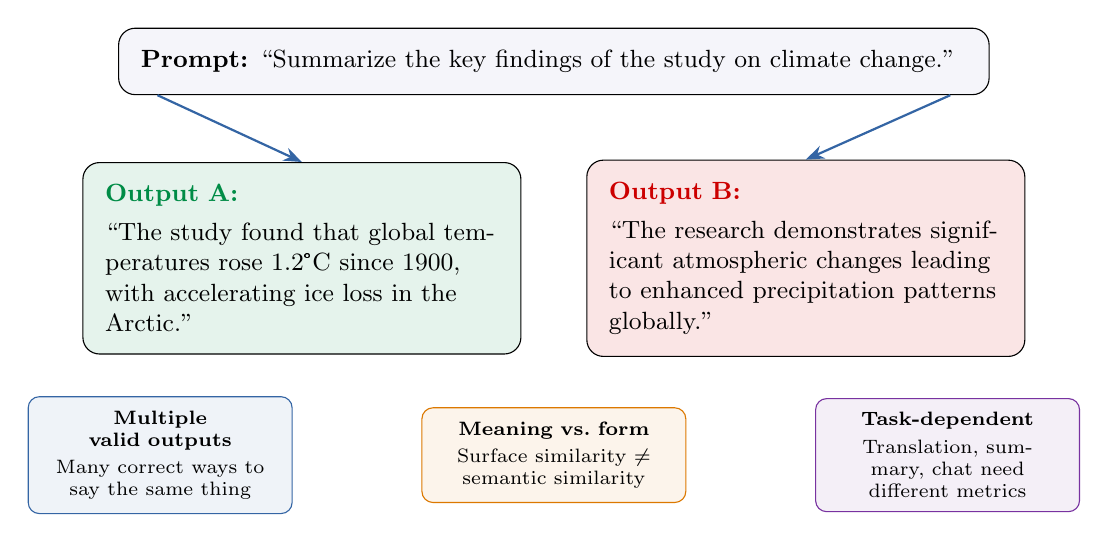
\begin{tikzpicture}
  % Prompt
  \node[draw, rounded corners=6pt, fill=lightbg, minimum width=10cm, align=center, inner sep=8pt, font=\small] (prompt) at (0, 3) {
    \textbf{Prompt:} ``Summarize the key findings of the study on climate change.''
  };

  % Output A
  \node[draw, rounded corners=6pt, fill=paramgreen!10, minimum width=5.5cm, text width=5cm, align=left, inner sep=8pt, font=\small] (outa) at (-3.2, 0.5) {
    \textbf{\textcolor{paramgreen}{Output A:}}\\[3pt]
    ``The study found that global temperatures rose 1.2\textdegree C since 1900, with accelerating ice loss in the Arctic.''
  };

  % Output B
  \node[draw, rounded corners=6pt, fill=sampred!10, minimum width=5.5cm, text width=5cm, align=left, inner sep=8pt, font=\small] (outb) at (3.2, 0.5) {
    \textbf{\textcolor{sampred}{Output B:}}\\[3pt]
    ``The research demonstrates significant atmospheric changes leading to enhanced precipitation patterns globally.''
  };

  \draw[-Stealth, thick, popblue] (prompt.south west) ++(0.5,0) -- (outa.north);
  \draw[-Stealth, thick, popblue] (prompt.south east) ++(-0.5,0) -- (outb.north);

  % Challenges
  \node[draw=popblue, fill=popblue!8, rounded corners=4pt, text width=3cm, align=center, inner sep=5pt, font=\scriptsize] at (-5, -2) {
    \textbf{Multiple valid outputs}\\[2pt]
    Many correct ways to say the same thing
  };
  \node[draw=orange1, fill=orange1!8, rounded corners=4pt, text width=3cm, align=center, inner sep=5pt, font=\scriptsize] at (0, -2) {
    \textbf{Meaning vs.\ form}\\[2pt]
    Surface similarity $\neq$ semantic similarity
  };
  \node[draw=violet1, fill=violet1!8, rounded corners=4pt, text width=3cm, align=center, inner sep=5pt, font=\scriptsize] at (5, -2) {
    \textbf{Task-dependent}\\[2pt]
    Translation, summary, chat need different metrics
  };
\end{tikzpicture}
\end{center}
\end{frame}

% ============================================================
% INTRINSIC VS EXTRINSIC
% ============================================================
\begin{frame}
\frametitle{Intrinsic vs.\ extrinsic evaluation}

\begin{center}
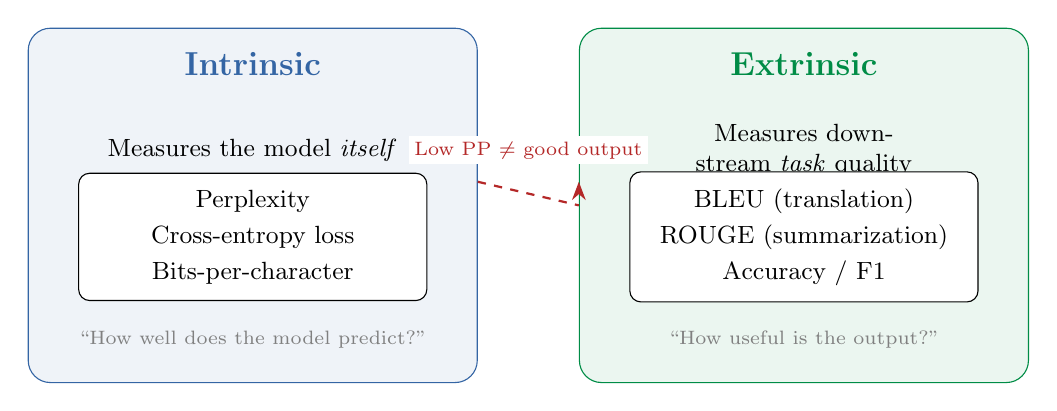
\begin{tikzpicture}
  % Intrinsic box
  \node[draw=popblue, fill=popblue!8, rounded corners=8pt, minimum width=5.5cm, minimum height=4.5cm, text width=5cm, align=center, inner sep=10pt] (intr) at (-3.5, 0) {};
  \node[font=\large\bfseries, text=popblue] at (-3.5, 1.8) {Intrinsic};
  \node[font=\small, text width=4.5cm, align=center] at (-3.5, 0.7) {
    Measures the model \emph{itself}
  };
  \node[draw, rounded corners=4pt, fill=white, inner sep=6pt, font=\small, text width=4cm, align=center] at (-3.5, -0.4) {
    Perplexity\\[2pt]
    Cross-entropy loss\\[2pt]
    Bits-per-character
  };
  \node[font=\scriptsize, text=gray] at (-3.5, -1.7) {``How well does the model predict?''};

  % Extrinsic box
  \node[draw=paramgreen, fill=paramgreen!8, rounded corners=8pt, minimum width=5.5cm, minimum height=4.5cm, text width=5cm, align=center, inner sep=10pt] (extr) at (3.5, 0) {};
  \node[font=\large\bfseries, text=paramgreen] at (3.5, 1.8) {Extrinsic};
  \node[font=\small, text width=4.5cm, align=center] at (3.5, 0.7) {
    Measures downstream \emph{task} quality
  };
  \node[draw, rounded corners=4pt, fill=white, inner sep=6pt, font=\small, text width=4cm, align=center] at (3.5, -0.4) {
    BLEU (translation)\\[2pt]
    ROUGE (summarization)\\[2pt]
    Accuracy / F1
  };
  \node[font=\scriptsize, text=gray] at (3.5, -1.7) {``How useful is the output?''};

  % Arrow between them
  \draw[-Stealth, thick, dashed, warnred] (intr.east) ++(0, 0.3) -- (extr.west) ++(0, 0.3);
  \node[font=\scriptsize, text=warnred, fill=white, inner sep=2pt] at (0, 0.7) {Low PP $\neq$ good output};
\end{tikzpicture}
\end{center}
\end{frame}

% ============================================================
% PERPLEXITY — DEFINITION
% ============================================================
\begin{frame}
\frametitle{Perplexity}

\vspace{-0.2cm}
\begin{center}
{\large
\[
\text{PP}(W) \;=\; \exp\!\Bigg(\!-\frac{1}{N}\sum_{i=1}^{N} \log P(w_i \mid w_{<i})\Bigg)
\]}
\end{center}

\vspace{-0.2cm}
\begin{center}
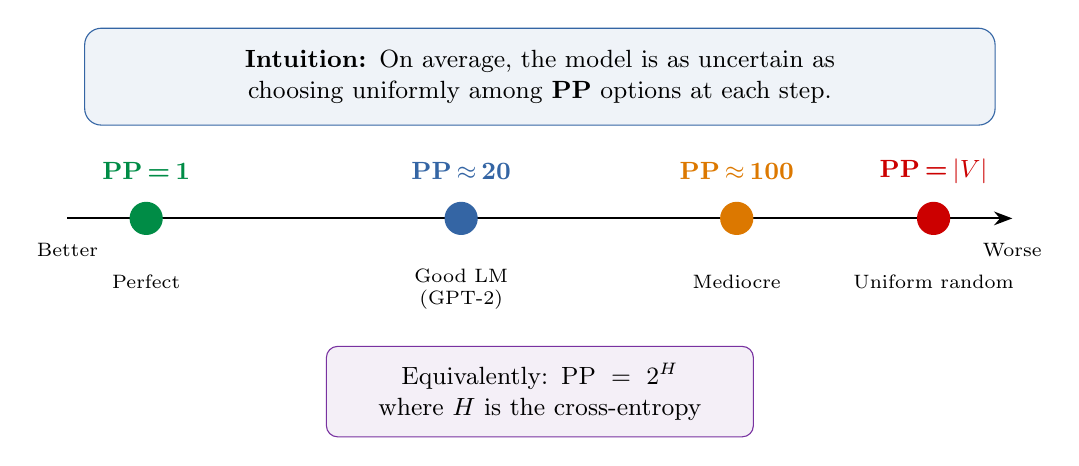
\begin{tikzpicture}
  % Intuition
  \node[draw=popblue, fill=popblue!8, rounded corners=6pt, text width=11cm, align=center, inner sep=8pt, font=\small] at (0, 1) {
    \textbf{Intuition:} On average, the model is as uncertain as choosing uniformly among \textbf{PP} options at each step.
  };

  % Scale bar
  \draw[thick, -Stealth] (-6, -0.8) -- (6, -0.8);
  \node[font=\scriptsize] at (-6, -1.2) {Better};
  \node[font=\scriptsize] at (6, -1.2) {Worse};

  % PP = 1
  \fill[paramgreen] (-5, -0.8) circle (6pt);
  \node[font=\small\bfseries, text=paramgreen] at (-5, -0.2) {PP\,=\,1};
  \node[font=\scriptsize] at (-5, -1.6) {Perfect};

  % PP ~ 10-30
  \fill[popblue] (-1, -0.8) circle (6pt);
  \node[font=\small\bfseries, text=popblue] at (-1, -0.2) {PP\,$\approx$\,20};
  \node[font=\scriptsize, text width=2cm, align=center] at (-1, -1.7) {Good LM\\(GPT-2)};

  % PP ~ 100
  \fill[orange1] (2.5, -0.8) circle (6pt);
  \node[font=\small\bfseries, text=orange1] at (2.5, -0.2) {PP\,$\approx$\,100};
  \node[font=\scriptsize] at (2.5, -1.6) {Mediocre};

  % PP = |V|
  \fill[sampred] (5, -0.8) circle (6pt);
  \node[font=\small\bfseries, text=sampred] at (5, -0.2) {PP\,=\,$|V|$};
  \node[font=\scriptsize] at (5, -1.6) {Uniform random};

  % Cross-entropy connection
  \node[draw=violet1, fill=violet1!8, rounded corners=4pt, inner sep=6pt, font=\small, text width=5cm, align=center] at (0, -3) {
    Equivalently: $\text{PP} = 2^{H}$ where $H$ is the cross-entropy
  };
\end{tikzpicture}
\end{center}
\end{frame}

% ============================================================
% PERPLEXITY — VISUAL INTUITION
% ============================================================
\begin{frame}
\frametitle{Perplexity --- visual intuition}

\begin{center}
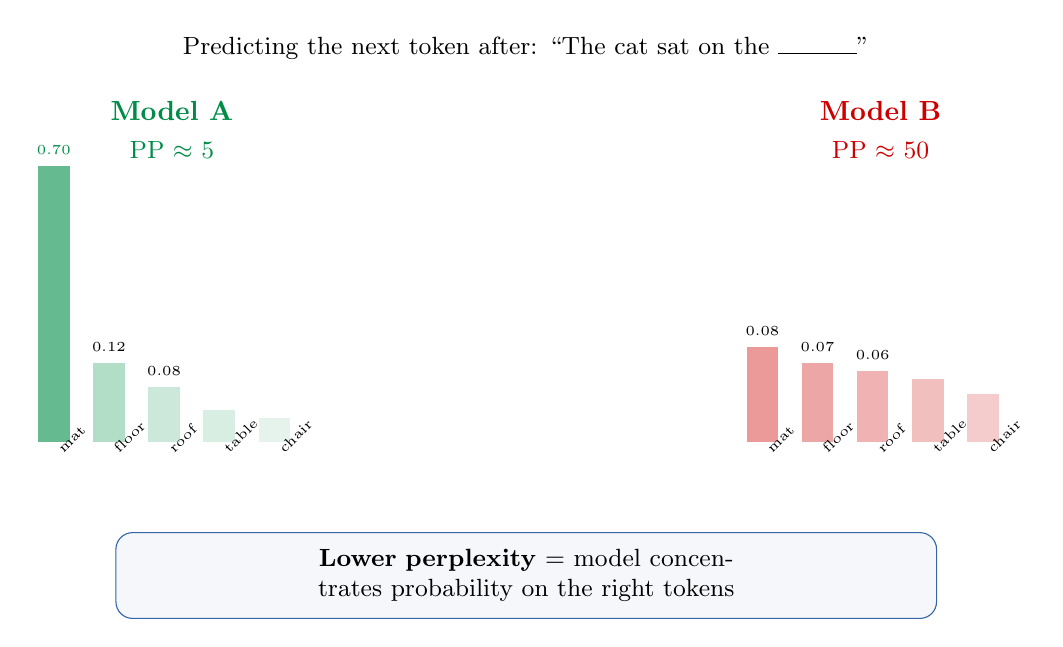
\begin{tikzpicture}
  % Context
  \node[font=\small] at (0, 3.5) {Predicting the next token after: ``The cat sat on the \rule{1cm}{0.4pt}''};

  % === Model A (left) ===
  \node[font=\normalsize\bfseries, text=paramgreen] at (-4.5, 2.7) {Model A};
  \node[font=\small, text=paramgreen] at (-4.5, 2.2) {PP $\approx$ 5};

  % Bars for Model A: peaked
  \fill[paramgreen!60] (-6.2, -1.5) rectangle (-5.8, 2.0);  % mat
  \fill[paramgreen!30] (-5.5, -1.5) rectangle (-5.1, -0.5);  % floor
  \fill[paramgreen!20] (-4.8, -1.5) rectangle (-4.4, -0.8);  % roof
  \fill[paramgreen!15] (-4.1, -1.5) rectangle (-3.7, -1.1);  % table
  \fill[paramgreen!10] (-3.4, -1.5) rectangle (-3.0, -1.2);  % chair

  % Labels
  \node[font=\tiny, rotate=45, anchor=west] at (-6.0, -1.7) {mat};
  \node[font=\tiny, rotate=45, anchor=west] at (-5.3, -1.7) {floor};
  \node[font=\tiny, rotate=45, anchor=west] at (-4.6, -1.7) {roof};
  \node[font=\tiny, rotate=45, anchor=west] at (-3.9, -1.7) {table};
  \node[font=\tiny, rotate=45, anchor=west] at (-3.2, -1.7) {chair};

  % Probability labels
  \node[font=\tiny, text=paramgreen] at (-6.0, 2.2) {0.70};
  \node[font=\tiny] at (-5.3, -0.3) {0.12};
  \node[font=\tiny] at (-4.6, -0.6) {0.08};

  % === Model B (right) ===
  \node[font=\normalsize\bfseries, text=sampred] at (4.5, 2.7) {Model B};
  \node[font=\small, text=sampred] at (4.5, 2.2) {PP $\approx$ 50};

  % Bars for Model B: flat
  \fill[sampred!40] (2.8, -1.5) rectangle (3.2, -0.3);  % mat
  \fill[sampred!35] (3.5, -1.5) rectangle (3.9, -0.5);  % floor
  \fill[sampred!30] (4.2, -1.5) rectangle (4.6, -0.6);  % roof
  \fill[sampred!25] (4.9, -1.5) rectangle (5.3, -0.7);  % table
  \fill[sampred!20] (5.6, -1.5) rectangle (6.0, -0.9);  % chair

  % Labels
  \node[font=\tiny, rotate=45, anchor=west] at (3.0, -1.7) {mat};
  \node[font=\tiny, rotate=45, anchor=west] at (3.7, -1.7) {floor};
  \node[font=\tiny, rotate=45, anchor=west] at (4.4, -1.7) {roof};
  \node[font=\tiny, rotate=45, anchor=west] at (5.1, -1.7) {table};
  \node[font=\tiny, rotate=45, anchor=west] at (5.8, -1.7) {chair};

  % Probability labels
  \node[font=\tiny] at (3.0, -0.1) {0.08};
  \node[font=\tiny] at (3.7, -0.3) {0.07};
  \node[font=\tiny] at (4.4, -0.4) {0.06};

  % Annotation
  \node[draw=popblue, fill=popblue!5, rounded corners=6pt, text width=10cm, align=center, inner sep=6pt, font=\small] at (0, -3.2) {
    \textbf{Lower perplexity} = model concentrates probability on the right tokens
  };
\end{tikzpicture}
\end{center}
\end{frame}

% ============================================================
% PERPLEXITY — CAVEATS
% ============================================================
\begin{frame}
\frametitle{Perplexity --- caveats}

\begin{center}
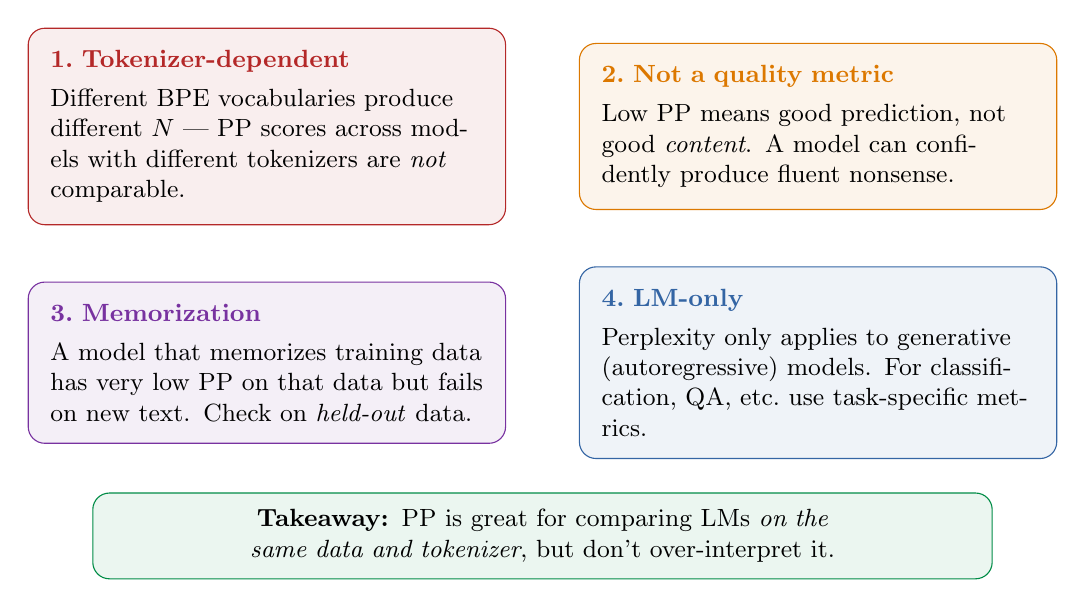
\begin{tikzpicture}
  % Warning boxes
  \node[draw=warnred, fill=warnred!8, rounded corners=6pt, text width=5.5cm, align=left, inner sep=8pt, font=\small] at (-3.5, 2) {
    \textbf{\textcolor{warnred}{1.~Tokenizer-dependent}}\\[3pt]
    Different BPE vocabularies produce different $N$ --- PP scores across models with different tokenizers are \emph{not} comparable.
  };

  \node[draw=orange1, fill=orange1!8, rounded corners=6pt, text width=5.5cm, align=left, inner sep=8pt, font=\small] at (3.5, 2) {
    \textbf{\textcolor{orange1}{2.~Not a quality metric}}\\[3pt]
    Low PP means good prediction, not good \emph{content}. A model can confidently produce fluent nonsense.
  };

  \node[draw=violet1, fill=violet1!8, rounded corners=6pt, text width=5.5cm, align=left, inner sep=8pt, font=\small] at (-3.5, -1) {
    \textbf{\textcolor{violet1}{3.~Memorization}}\\[3pt]
    A model that memorizes training data has very low PP on that data but fails on new text. Check on \emph{held-out} data.
  };

  \node[draw=popblue, fill=popblue!8, rounded corners=6pt, text width=5.5cm, align=left, inner sep=8pt, font=\small] at (3.5, -1) {
    \textbf{\textcolor{popblue}{4.~LM-only}}\\[3pt]
    Perplexity only applies to generative (autoregressive) models. For classification, QA, etc.\ use task-specific metrics.
  };

  % Bottom takeaway
  \node[draw=paramgreen, fill=paramgreen!8, rounded corners=6pt, text width=11cm, align=center, inner sep=6pt, font=\small] at (0, -3.2) {
    \textbf{Takeaway:} PP is great for comparing LMs \emph{on the same data and tokenizer}, but don't over-interpret it.
  };
\end{tikzpicture}
\end{center}
\end{frame}

% ============================================================
% BLEU — DEFINITION
% ============================================================
\begin{frame}
\frametitle{BLEU --- Bilingual Evaluation Understudy}

\vspace{-0.1cm}
\begin{center}
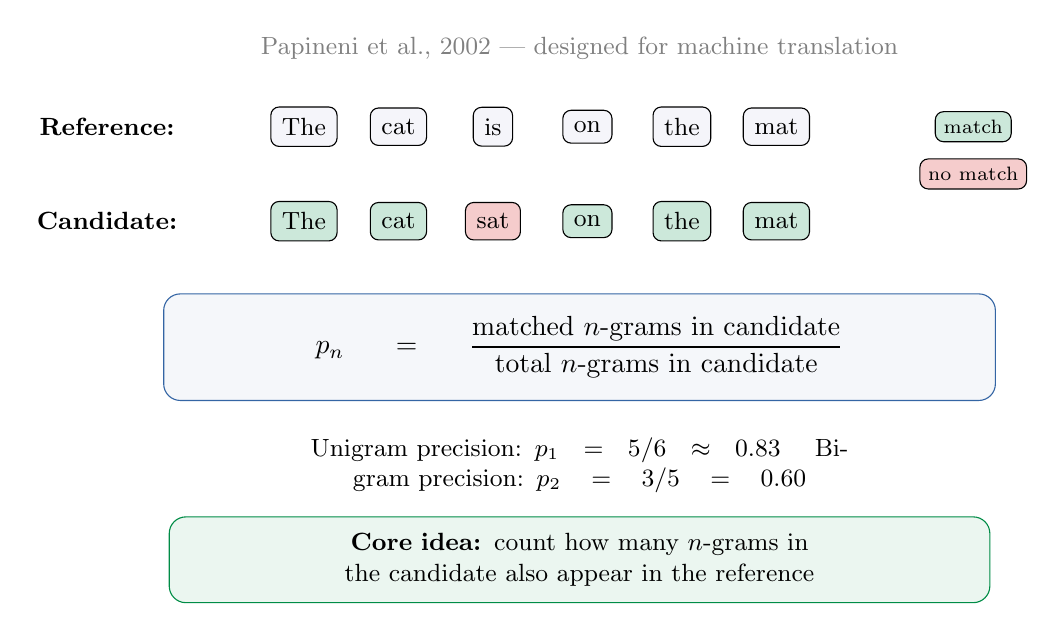
\begin{tikzpicture}
  % Context
  \node[font=\small, text=gray] at (0, 3.5) {Papineni et al., 2002 --- designed for machine translation};

  % Reference
  \node[font=\small\bfseries] at (-6, 2.5) {Reference:};
  \node[draw, rounded corners=3pt, fill=lightbg, inner sep=4pt, font=\small] (r1) at (-3.5, 2.5) {The};
  \node[draw, rounded corners=3pt, fill=lightbg, inner sep=4pt, font=\small] (r2) at (-2.3, 2.5) {cat};
  \node[draw, rounded corners=3pt, fill=lightbg, inner sep=4pt, font=\small] (r3) at (-1.1, 2.5) {is};
  \node[draw, rounded corners=3pt, fill=lightbg, inner sep=4pt, font=\small] (r4) at (0.1, 2.5) {on};
  \node[draw, rounded corners=3pt, fill=lightbg, inner sep=4pt, font=\small] (r5) at (1.3, 2.5) {the};
  \node[draw, rounded corners=3pt, fill=lightbg, inner sep=4pt, font=\small] (r6) at (2.5, 2.5) {mat};

  % Candidate
  \node[font=\small\bfseries] at (-6, 1.3) {Candidate:};
  \node[draw, rounded corners=3pt, fill=paramgreen!20, inner sep=4pt, font=\small] (c1) at (-3.5, 1.3) {The};
  \node[draw, rounded corners=3pt, fill=paramgreen!20, inner sep=4pt, font=\small] (c2) at (-2.3, 1.3) {cat};
  \node[draw, rounded corners=3pt, fill=sampred!20, inner sep=4pt, font=\small] (c3) at (-1.1, 1.3) {sat};
  \node[draw, rounded corners=3pt, fill=paramgreen!20, inner sep=4pt, font=\small] (c4) at (0.1, 1.3) {on};
  \node[draw, rounded corners=3pt, fill=paramgreen!20, inner sep=4pt, font=\small] (c5) at (1.3, 1.3) {the};
  \node[draw, rounded corners=3pt, fill=paramgreen!20, inner sep=4pt, font=\small] (c6) at (2.5, 1.3) {mat};

  % Legend
  \node[draw, rounded corners=3pt, fill=paramgreen!20, inner sep=3pt, font=\scriptsize] at (5, 2.5) {match};
  \node[draw, rounded corners=3pt, fill=sampred!20, inner sep=3pt, font=\scriptsize] at (5, 1.9) {no match};

  % Precision formula
  \node[draw=popblue, fill=popblue!5, rounded corners=6pt, text width=10cm, align=center, inner sep=8pt] at (0, -0.3) {
    {\normalsize $\displaystyle p_n \;=\; \frac{\text{matched $n$-grams in candidate}}{\text{total $n$-grams in candidate}}$}
  };

  % Example counts
  \node[font=\small, text width=10cm, align=center] at (0, -1.8) {
    Unigram precision: $p_1 = 5/6 \approx 0.83$ \quad
    Bigram precision: $p_2 = 3/5 = 0.60$
  };

  % Key idea
  \node[draw=paramgreen, fill=paramgreen!8, rounded corners=6pt, text width=10cm, align=center, inner sep=6pt, font=\small] at (0, -3) {
    \textbf{Core idea:} count how many $n$-grams in the candidate also appear in the reference
  };
\end{tikzpicture}
\end{center}
\end{frame}

% ============================================================
% BLEU — MODIFIED PRECISION & BP
% ============================================================
\begin{frame}
\frametitle{BLEU --- modified precision \& brevity penalty}

\vspace{-0.2cm}
\begin{center}
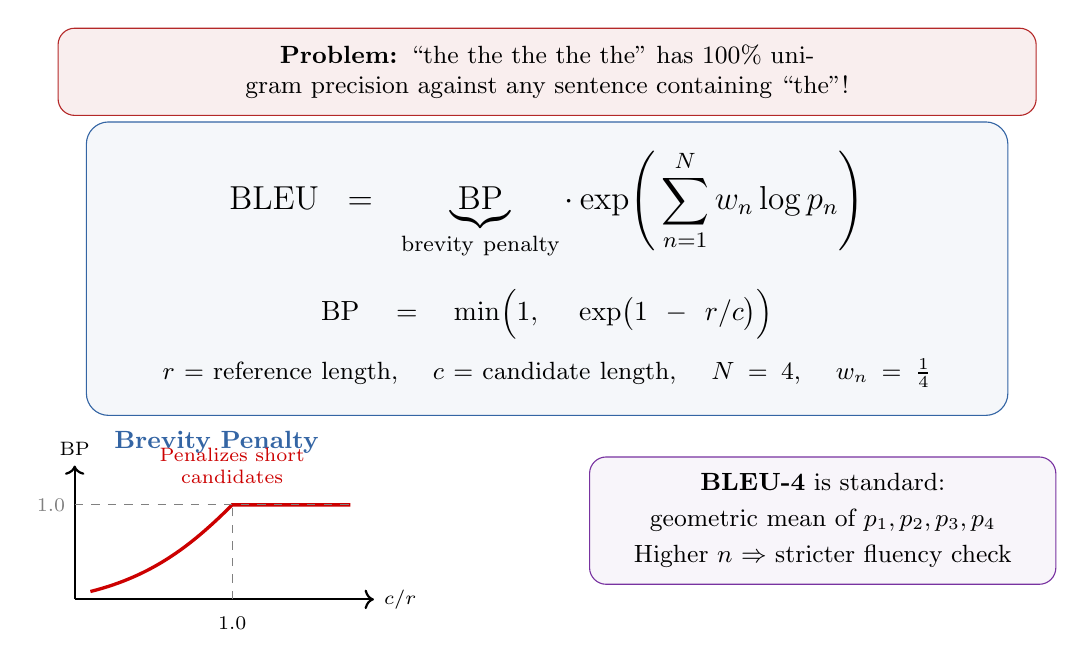
\begin{tikzpicture}
  % Problem
  \node[draw=warnred, fill=warnred!8, rounded corners=6pt, text width=12cm, align=center, inner sep=6pt, font=\small] at (0, 3.2) {
    \textbf{Problem:} ``the the the the the'' has 100\% unigram precision against any sentence containing ``the''!
  };

  % Solution: clipped counts
  \node[font=\small, text width=12cm, align=center] at (0, 2.2) {
    \textbf{Fix:} clip each $n$-gram count to its max occurrence in any reference
  };

  % BLEU formula
  \node[draw=popblue, fill=popblue!5, rounded corners=8pt, inner sep=10pt, text width=11cm, align=center] at (0, 0.7) {
    {\large $\displaystyle \text{BLEU} = \underbrace{\text{BP}}_{\text{brevity penalty}} \cdot \exp\!\Bigg(\sum_{n=1}^{N} w_n \log p_n\Bigg)$}\\[10pt]
    {\normalsize $\displaystyle \text{BP} = \min\!\Big(1,\; \exp\!\big(1 - r/c\big)\Big)$}\\[6pt]
    {\small $r$ = reference length, \quad $c$ = candidate length, \quad $N=4$, \quad $w_n = \tfrac{1}{4}$}
  };

  % BP curve (manual)
  \node[font=\small\bfseries, text=popblue] at (-4.2, -1.5) {Brevity Penalty};
  \draw[thick, ->] (-6, -3.5) -- (-2.2, -3.5) node[right, font=\scriptsize] {$c/r$};
  \draw[thick, ->] (-6, -3.5) -- (-6, -1.8) node[above, font=\scriptsize] {BP};

  % BP curve: exponential rise then flat at 1
  \draw[very thick, sampred] (-5.8, -3.4) .. controls (-5.0, -3.2) and (-4.5, -2.8) .. (-4, -2.3) -- (-2.5, -2.3);
  \draw[dashed, gray] (-6, -2.3) -- (-2.5, -2.3);
  \node[font=\scriptsize, text=gray] at (-6.3, -2.3) {1.0};
  \node[font=\scriptsize] at (-4, -3.8) {1.0};
  \draw[dashed, gray] (-4, -3.5) -- (-4, -2.3);

  % Annotation
  \node[font=\scriptsize, text=sampred, text width=3cm, align=center] at (-4, -1.8) {Penalizes short candidates};

  % Why N=4
  \node[draw=violet1, fill=violet1!5, rounded corners=6pt, text width=5.5cm, align=center, inner sep=6pt, font=\small] at (3.5, -2.5) {
    \textbf{BLEU-4} is standard:\\[2pt]
    geometric mean of $p_1, p_2, p_3, p_4$\\[2pt]
    Higher $n$ $\Rightarrow$ stricter fluency check
  };
\end{tikzpicture}
\end{center}
\end{frame}

% ============================================================
% BLEU — WORKED EXAMPLE
% ============================================================
\begin{frame}
\frametitle{BLEU --- worked example}

\vspace{-0.2cm}
\begin{center}
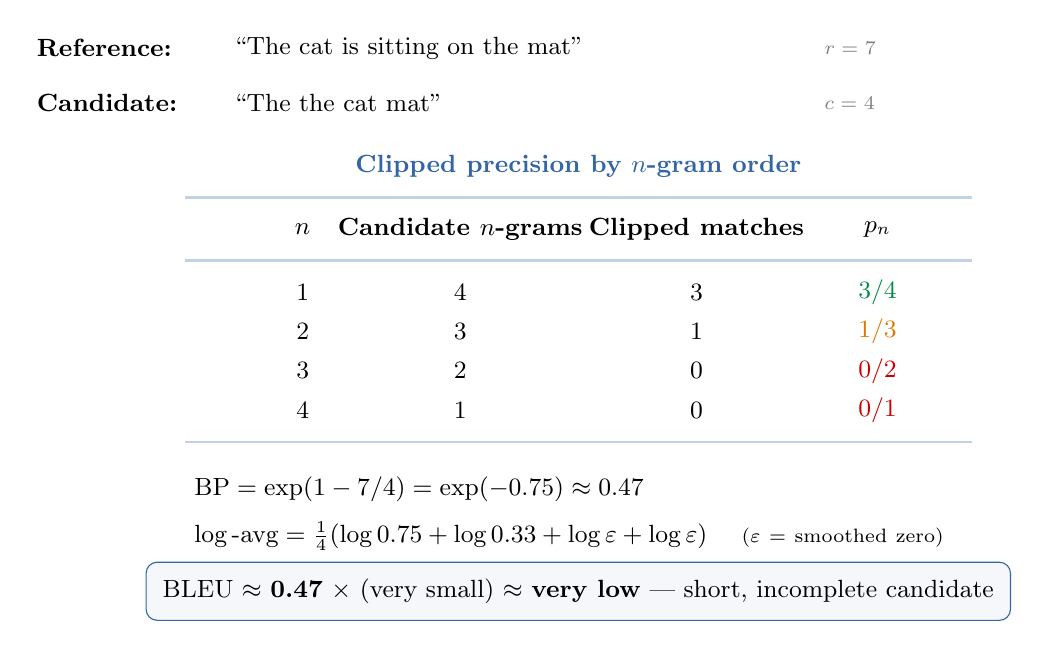
\begin{tikzpicture}
  % Sentences
  \node[font=\small\bfseries, anchor=west] at (-7, 3.3) {Reference:};
  \node[font=\small, anchor=west] at (-4.5, 3.3) {``The cat is sitting on the mat''};
  \node[font=\small\bfseries, anchor=west] at (-7, 2.6) {Candidate:};
  \node[font=\small, anchor=west] at (-4.5, 2.6) {``The the cat mat''};

  % Lengths
  \node[font=\scriptsize, text=gray, anchor=west] at (3, 3.3) {$r = 7$};
  \node[font=\scriptsize, text=gray, anchor=west] at (3, 2.6) {$c = 4$};

  % N-gram table
  \node[font=\small\bfseries, text=popblue] at (0, 1.8) {Clipped precision by $n$-gram order};

  \draw[thick, popblue!30] (-5, 1.4) -- (5, 1.4);

  % Headers
  \node[font=\small\bfseries] at (-3.5, 1.0) {$n$};
  \node[font=\small\bfseries] at (-1.5, 1.0) {Candidate $n$-grams};
  \node[font=\small\bfseries] at (1.5, 1.0) {Clipped matches};
  \node[font=\small\bfseries] at (3.8, 1.0) {$p_n$};

  \draw[thick, popblue!30] (-5, 0.6) -- (5, 0.6);

  % Row 1
  \node[font=\small] at (-3.5, 0.2) {1};
  \node[font=\small] at (-1.5, 0.2) {4};
  \node[font=\small] at (1.5, 0.2) {3};
  \node[font=\small, text=paramgreen] at (3.8, 0.2) {3/4};

  % Row 2
  \node[font=\small] at (-3.5, -0.3) {2};
  \node[font=\small] at (-1.5, -0.3) {3};
  \node[font=\small] at (1.5, -0.3) {1};
  \node[font=\small, text=orange1] at (3.8, -0.3) {1/3};

  % Row 3
  \node[font=\small] at (-3.5, -0.8) {3};
  \node[font=\small] at (-1.5, -0.8) {2};
  \node[font=\small] at (1.5, -0.8) {0};
  \node[font=\small, text=sampred] at (3.8, -0.8) {0/2};

  % Row 4
  \node[font=\small] at (-3.5, -1.3) {4};
  \node[font=\small] at (-1.5, -1.3) {1};
  \node[font=\small] at (1.5, -1.3) {0};
  \node[font=\small, text=sampred] at (3.8, -1.3) {0/1};

  \draw[thick, popblue!30] (-5, -1.7) -- (5, -1.7);

  % Computation
  \node[font=\small, text width=10cm, align=left, anchor=west] at (-5, -2.3) {
    $\text{BP} = \exp(1 - 7/4) = \exp(-0.75) \approx 0.47$
  };
  \node[font=\small, text width=10cm, align=left, anchor=west] at (-5, -2.9) {
    $\log\text{-avg} = \tfrac{1}{4}(\log 0.75 + \log 0.33 + \log \varepsilon + \log \varepsilon)$ \quad {\scriptsize ($\varepsilon$ = smoothed zero)}
  };
  \node[draw=popblue, fill=popblue!5, rounded corners=4pt, inner sep=6pt, font=\small] at (0, -3.6) {
    BLEU $\approx$ \textbf{0.47} $\times$ (very small) $\approx$ \textbf{very low} --- short, incomplete candidate
  };
\end{tikzpicture}
\end{center}
\end{frame}

% ============================================================
% ROUGE — DEFINITION
% ============================================================
\begin{frame}
\frametitle{ROUGE --- Recall-Oriented Understudy for Gisting Evaluation}

\vspace{-0.1cm}
\begin{center}
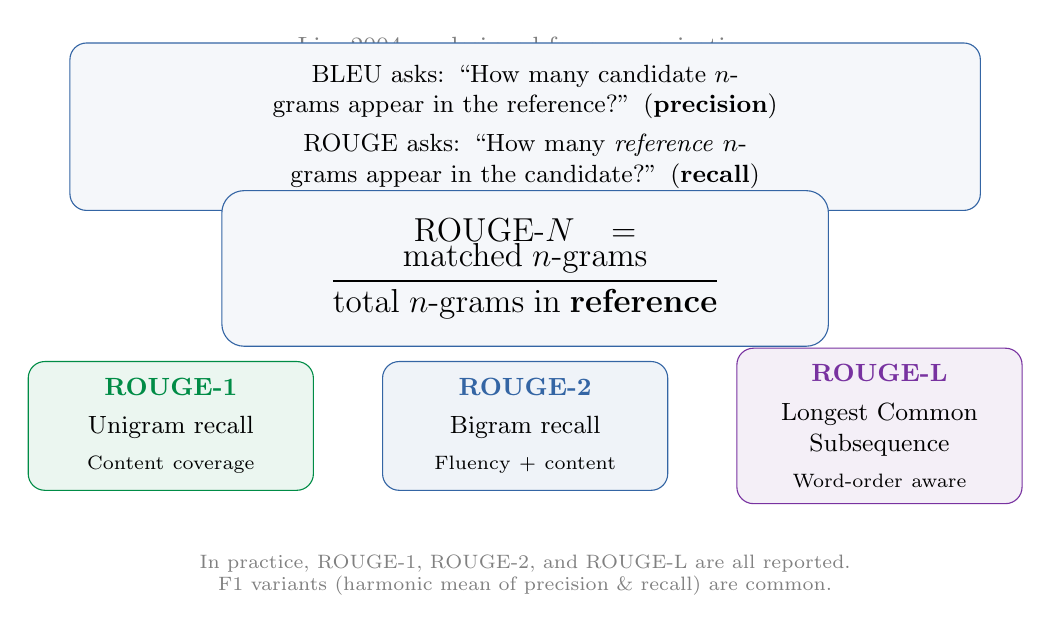
\begin{tikzpicture}
  % Context
  \node[font=\small, text=gray] at (0, 3.5) {Lin, 2004 --- designed for summarization};

  % Key difference
  \node[draw=popblue, fill=popblue!5, rounded corners=6pt, text width=11cm, align=center, inner sep=8pt, font=\small] at (0, 2.5) {
    BLEU asks: ``How many candidate $n$-grams appear in the reference?'' (\textbf{precision})\\[3pt]
    ROUGE asks: ``How many \emph{reference} $n$-grams appear in the candidate?'' (\textbf{recall})
  };

  % Formula
  \node[draw=popblue, fill=popblue!5, rounded corners=8pt, inner sep=10pt, text width=7cm, align=center] at (0, 0.7) {
    {\large $\displaystyle \text{ROUGE-}N = \frac{\text{matched $n$-grams}}{\text{total $n$-grams in \textbf{reference}}}$}
  };

  % Three variants
  \node[draw=paramgreen, fill=paramgreen!8, rounded corners=6pt, text width=3.2cm, align=center, inner sep=6pt, font=\small] at (-4.5, -1.3) {
    \textbf{\textcolor{paramgreen}{ROUGE-1}}\\[3pt]
    Unigram recall\\[2pt]
    {\scriptsize Content coverage}
  };
  \node[draw=popblue, fill=popblue!8, rounded corners=6pt, text width=3.2cm, align=center, inner sep=6pt, font=\small] at (0, -1.3) {
    \textbf{\textcolor{popblue}{ROUGE-2}}\\[3pt]
    Bigram recall\\[2pt]
    {\scriptsize Fluency + content}
  };
  \node[draw=violet1, fill=violet1!8, rounded corners=6pt, text width=3.2cm, align=center, inner sep=6pt, font=\small] at (4.5, -1.3) {
    \textbf{\textcolor{violet1}{ROUGE-L}}\\[3pt]
    Longest Common\\Subsequence\\[2pt]
    {\scriptsize Word-order aware}
  };

  % Note
  \node[font=\scriptsize, text=gray, text width=10cm, align=center] at (0, -3.2) {
    In practice, ROUGE-1, ROUGE-2, and ROUGE-L are all reported. F1 variants (harmonic mean of precision \& recall) are common.
  };
\end{tikzpicture}
\end{center}
\end{frame}

% ============================================================
% ROUGE vs BLEU
% ============================================================
\begin{frame}
\frametitle{BLEU vs.\ ROUGE}

\vspace{-0.1cm}
\begin{center}
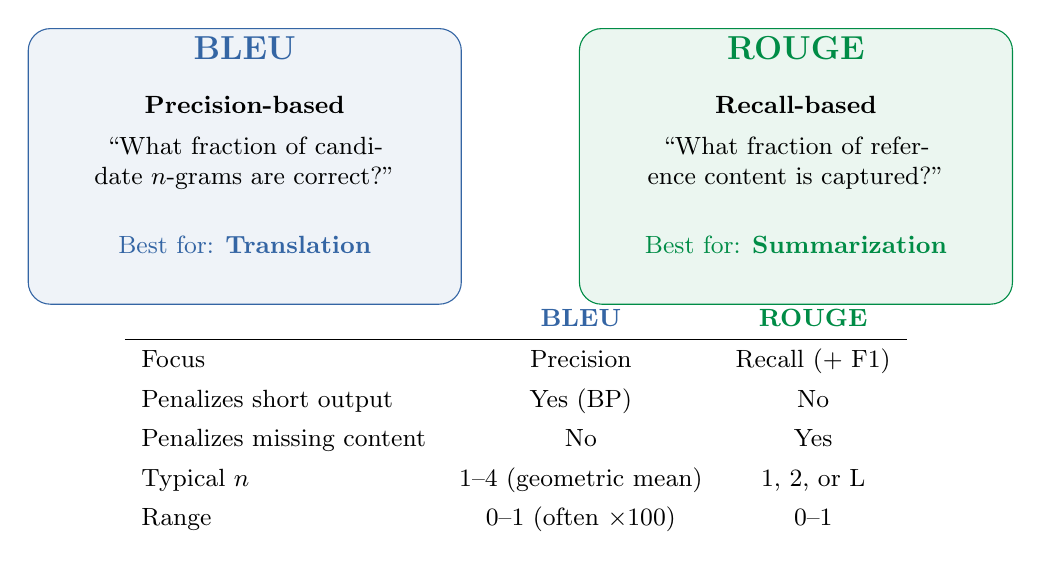
\begin{tikzpicture}
  % BLEU side
  \node[draw=popblue, fill=popblue!8, rounded corners=8pt, minimum width=5.5cm, minimum height=3.5cm, inner sep=10pt] at (-3.5, 1.2) {};
  \node[font=\large\bfseries, text=popblue] at (-3.5, 2.7) {BLEU};
  \node[font=\small, text width=4.8cm, align=center] at (-3.5, 1.5) {
    \textbf{Precision-based}\\[4pt]
    ``What fraction of candidate $n$-grams are correct?''
  };
  \node[font=\small, text=popblue] at (-3.5, 0.2) {Best for: \textbf{Translation}};

  % ROUGE side
  \node[draw=paramgreen, fill=paramgreen!8, rounded corners=8pt, minimum width=5.5cm, minimum height=3.5cm, inner sep=10pt] at (3.5, 1.2) {};
  \node[font=\large\bfseries, text=paramgreen] at (3.5, 2.7) {ROUGE};
  \node[font=\small, text width=4.8cm, align=center] at (3.5, 1.5) {
    \textbf{Recall-based}\\[4pt]
    ``What fraction of reference content is captured?''
  };
  \node[font=\small, text=paramgreen] at (3.5, 0.2) {Best for: \textbf{Summarization}};

  % Comparison table
  \renewcommand{\arraystretch}{1.3}
  \node at (0, -2) {
    {\small
    \begin{tabular}{l c c}
      & \textbf{\textcolor{popblue}{BLEU}} & \textbf{\textcolor{paramgreen}{ROUGE}} \\
      \hline
      Focus & Precision & Recall (+ F1) \\
      Penalizes short output & Yes (BP) & No \\
      Penalizes missing content & No & Yes \\
      Typical $n$ & 1--4 (geometric mean) & 1, 2, or L \\
      Range & 0--1 (often $\times 100$) & 0--1 \\
    \end{tabular}
    }
  };
\end{tikzpicture}
\end{center}
\end{frame}

% ============================================================
% LIMITATIONS OF N-GRAM METRICS
% ============================================================
\begin{frame}
\frametitle{Limitations of $n$-gram metrics}

\begin{center}
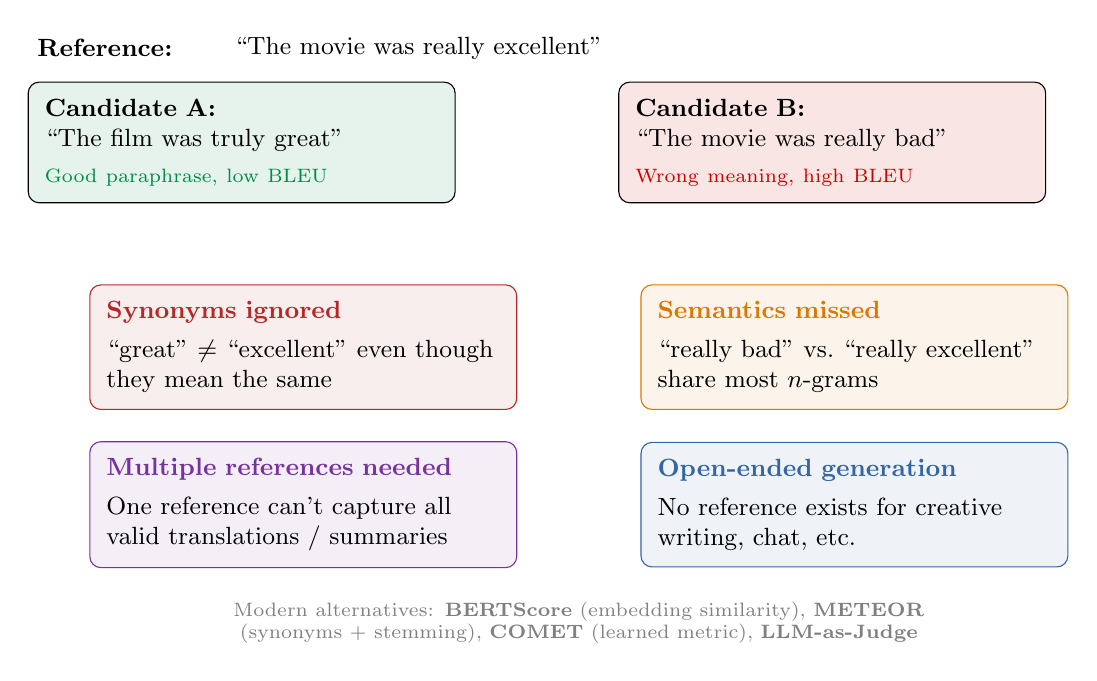
\begin{tikzpicture}
  % Example
  \node[font=\small\bfseries, anchor=west] at (-7, 3.3) {Reference:};
  \node[font=\small, anchor=west] at (-4.5, 3.3) {``The movie was really excellent''};

  \node[draw, rounded corners=4pt, fill=paramgreen!10, text width=5cm, align=left, inner sep=6pt, font=\small, anchor=west] at (-7, 2.1) {
    \textbf{Candidate A:}\\
    ``The film was truly great''\\[2pt]
    {\scriptsize \textcolor{paramgreen}{Good paraphrase, low BLEU}}
  };
  \node[draw, rounded corners=4pt, fill=sampred!10, text width=5cm, align=left, inner sep=6pt, font=\small, anchor=west] at (0.5, 2.1) {
    \textbf{Candidate B:}\\
    ``The movie was really bad''\\[2pt]
    {\scriptsize \textcolor{sampred}{Wrong meaning, high BLEU}}
  };

  % Issues
  \node[draw=warnred, fill=warnred!8, rounded corners=4pt, text width=5cm, align=left, inner sep=6pt, font=\small] at (-3.5, -0.5) {
    \textbf{\textcolor{warnred}{Synonyms ignored}}\\[3pt]
    ``great'' $\neq$ ``excellent'' even though they mean the same
  };
  \node[draw=orange1, fill=orange1!8, rounded corners=4pt, text width=5cm, align=left, inner sep=6pt, font=\small] at (3.5, -0.5) {
    \textbf{\textcolor{orange1}{Semantics missed}}\\[3pt]
    ``really bad'' vs.\ ``really excellent'' share most $n$-grams
  };
  \node[draw=violet1, fill=violet1!8, rounded corners=4pt, text width=5cm, align=left, inner sep=6pt, font=\small] at (-3.5, -2.5) {
    \textbf{\textcolor{violet1}{Multiple references needed}}\\[3pt]
    One reference can't capture all valid translations / summaries
  };
  \node[draw=popblue, fill=popblue!8, rounded corners=4pt, text width=5cm, align=left, inner sep=6pt, font=\small] at (3.5, -2.5) {
    \textbf{\textcolor{popblue}{Open-ended generation}}\\[3pt]
    No reference exists for creative writing, chat, etc.
  };

  % Alternatives
  \node[font=\scriptsize, text=gray, text width=12cm, align=center] at (0, -4) {
    Modern alternatives: \textbf{BERTScore} (embedding similarity), \textbf{METEOR} (synonyms + stemming), \textbf{COMET} (learned metric), \textbf{LLM-as-Judge}
  };
\end{tikzpicture}
\end{center}
\end{frame}

% ============================================================
% BENCHMARKS — OVERVIEW
% ============================================================
\begin{frame}
\frametitle{Benchmarks --- evaluating holistically}

\begin{center}
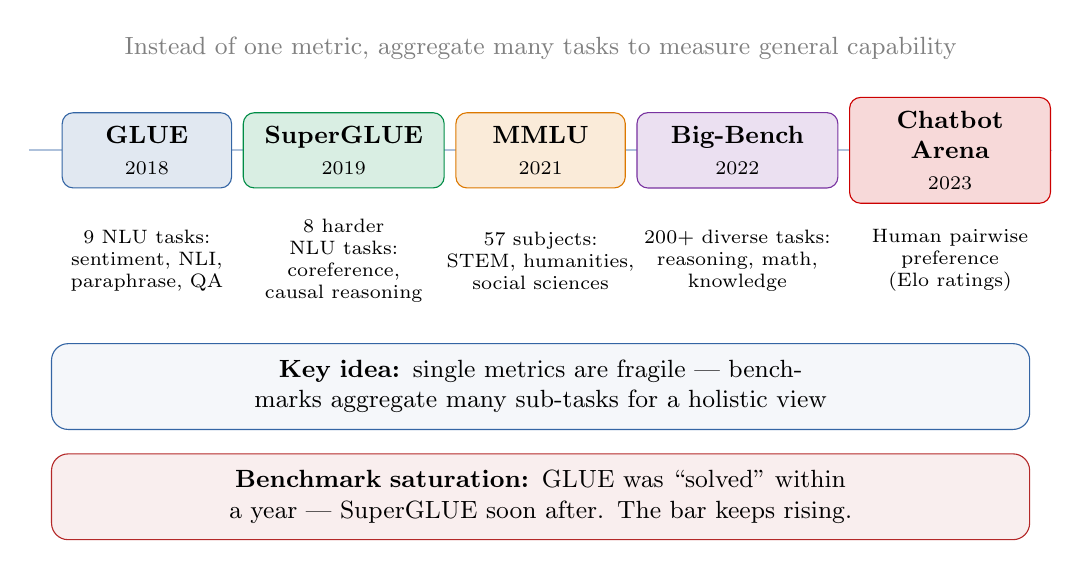
\begin{tikzpicture}
  % Title idea
  \node[font=\small, text=gray, text width=12cm, align=center] at (0, 3.5) {
    Instead of one metric, aggregate many tasks to measure general capability
  };

  % Timeline
  \draw[thick, -Stealth, popblue!40] (-6.5, 2.2) -- (6.5, 2.2);

  % GLUE
  \node[draw=popblue, fill=popblue!15, rounded corners=4pt, inner sep=5pt, font=\small, text width=1.8cm, align=center] (glue) at (-5, 2.2) {
    \textbf{GLUE}\\{\scriptsize 2018}
  };

  % SuperGLUE
  \node[draw=paramgreen, fill=paramgreen!15, rounded corners=4pt, inner sep=5pt, font=\small, text width=2.2cm, align=center] (sglue) at (-2.5, 2.2) {
    \textbf{SuperGLUE}\\{\scriptsize 2019}
  };

  % MMLU
  \node[draw=orange1, fill=orange1!15, rounded corners=4pt, inner sep=5pt, font=\small, text width=1.8cm, align=center] (mmlu) at (0, 2.2) {
    \textbf{MMLU}\\{\scriptsize 2021}
  };

  % Big-Bench
  \node[draw=violet1, fill=violet1!15, rounded corners=4pt, inner sep=5pt, font=\small, text width=2.2cm, align=center] (bb) at (2.5, 2.2) {
    \textbf{Big-Bench}\\{\scriptsize 2022}
  };

  % LMSYS
  \node[draw=sampred, fill=sampred!15, rounded corners=4pt, inner sep=5pt, font=\small, text width=2.2cm, align=center] (arena) at (5.2, 2.2) {
    \textbf{Chatbot Arena}\\{\scriptsize 2023}
  };

  % Descriptions below
  \node[font=\scriptsize, text width=2.5cm, align=center] at (-5, 0.8) {
    9 NLU tasks:\\sentiment, NLI,\\paraphrase, QA
  };
  \node[font=\scriptsize, text width=2.5cm, align=center] at (-2.5, 0.8) {
    8 harder NLU tasks:\\coreference,\\causal reasoning
  };
  \node[font=\scriptsize, text width=2.5cm, align=center] at (0, 0.8) {
    57 subjects:\\STEM, humanities,\\social sciences
  };
  \node[font=\scriptsize, text width=2.5cm, align=center] at (2.5, 0.8) {
    200+ diverse tasks:\\reasoning, math,\\knowledge
  };
  \node[font=\scriptsize, text width=2.5cm, align=center] at (5.2, 0.8) {
    Human pairwise\\preference\\(Elo ratings)
  };

  % Key insight
  \node[draw=popblue, fill=popblue!5, rounded corners=6pt, text width=12cm, align=center, inner sep=6pt, font=\small] at (0, -0.8) {
    \textbf{Key idea:} single metrics are fragile --- benchmarks aggregate many sub-tasks for a holistic view
  };

  % Saturation warning
  \node[draw=warnred, fill=warnred!8, rounded corners=6pt, text width=12cm, align=center, inner sep=6pt, font=\small] at (0, -2.2) {
    \textbf{Benchmark saturation:} GLUE was ``solved'' within a year --- SuperGLUE soon after. The bar keeps rising.
  };
\end{tikzpicture}
\end{center}
\end{frame}

% ============================================================
% KEY BENCHMARKS TABLE
% ============================================================
\begin{frame}
\frametitle{Key benchmarks at a glance}

\vspace{-0.1cm}
\renewcommand{\arraystretch}{1.4}
\begin{center}
{\small
\begin{tabular}{>{\bfseries}l l l l}
  \textbf{Benchmark} & \textbf{What it tests} & \textbf{Format} & \textbf{Notable for} \\
  \hline
  \textcolor{popblue}{MMLU} & Knowledge (57 subjects) & Multiple choice & Breadth of knowledge \\[2pt]
  \textcolor{paramgreen}{HumanEval} & Code generation & Function completion & Coding ability \\[2pt]
  \textcolor{orange1}{HellaSwag} & Commonsense reasoning & Sentence completion & Physical understanding \\[2pt]
  \textcolor{violet1}{TruthfulQA} & Factual accuracy & QA & Hallucination resistance \\[2pt]
  \textcolor{sampred}{GSM8K} & Math reasoning & Word problems & Step-by-step reasoning \\[2pt]
  \textcolor{popblue}{ARC} & Science questions & Multiple choice & Grade-school science \\[2pt]
  \textcolor{paramgreen}{Winogrande} & Coreference & Pronoun resolution & Linguistic understanding \\
  \hline
\end{tabular}
}
\end{center}

\vspace{0.3cm}
\begin{center}

\begin{tikzpicture}
  % Leaderboard mockup
  \node[draw=popblue, fill=popblue!5, rounded corners=6pt, text width=10cm, align=center, inner sep=8pt, font=\small] at (0, 0) {
    Aggregate scores (e.g., \textbf{Open LLM Leaderboard}) let you compare models at a glance---\\
    but no single number tells the full story.
  };
\end{tikzpicture}
\end{center}
\end{frame}

% ============================================================
% THE EVALUATION LANDSCAPE
% ============================================================
\begin{frame}
\frametitle{The evaluation landscape}

\begin{center}
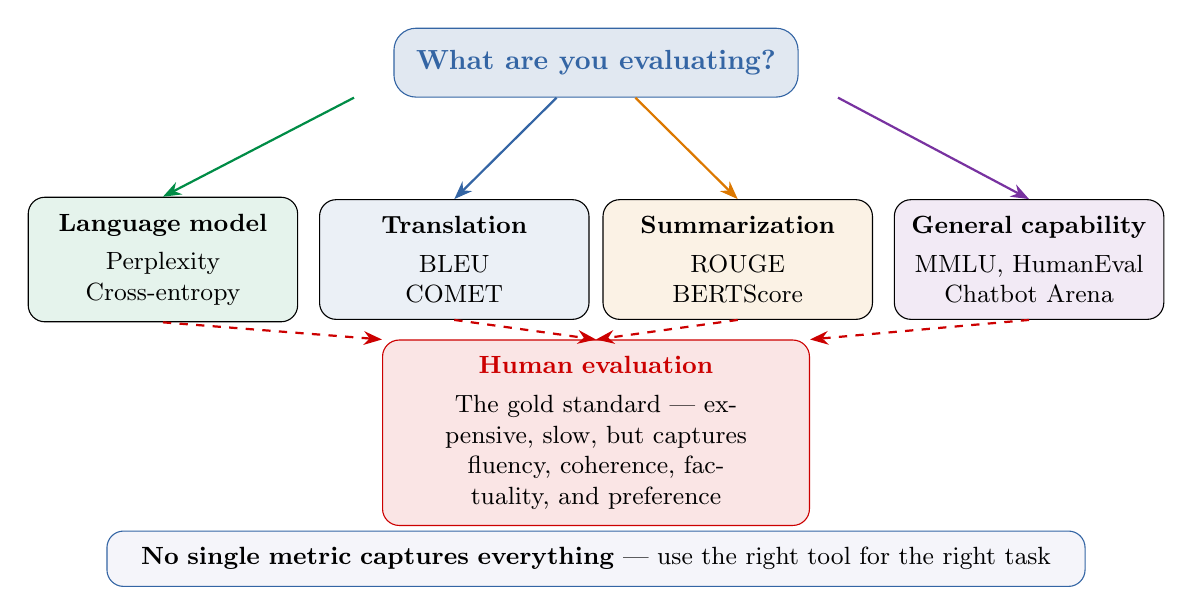
\begin{tikzpicture}
  % Central question
  \node[draw=popblue, fill=popblue!15, rounded corners=8pt, font=\normalsize\bfseries, inner sep=8pt, text=popblue] (center) at (0, 2.5) {What are you evaluating?};

  % Branches
  \node[draw, rounded corners=6pt, fill=paramgreen!10, text width=3cm, align=center, inner sep=6pt, font=\small] (lm) at (-5.5, 0) {
    \textbf{Language model}\\[3pt]
    Perplexity\\Cross-entropy
  };
  \node[draw, rounded corners=6pt, fill=popblue!10, text width=3cm, align=center, inner sep=6pt, font=\small] (trans) at (-1.8, 0) {
    \textbf{Translation}\\[3pt]
    BLEU\\COMET
  };
  \node[draw, rounded corners=6pt, fill=orange1!10, text width=3cm, align=center, inner sep=6pt, font=\small] (summ) at (1.8, 0) {
    \textbf{Summarization}\\[3pt]
    ROUGE\\BERTScore
  };
  \node[draw, rounded corners=6pt, fill=violet1!10, text width=3cm, align=center, inner sep=6pt, font=\small] (gen) at (5.5, 0) {
    \textbf{General capability}\\[3pt]
    MMLU, HumanEval\\Chatbot Arena
  };

  % Arrows from center
  \draw[-Stealth, thick, paramgreen] (center.south west) ++(-0.5, 0) -- (lm.north);
  \draw[-Stealth, thick, popblue] (center.south) ++(-0.5, 0) -- (trans.north);
  \draw[-Stealth, thick, orange1] (center.south) ++(0.5, 0) -- (summ.north);
  \draw[-Stealth, thick, violet1] (center.south east) ++(0.5, 0) -- (gen.north);

  % Human evaluation
  \node[draw=sampred, fill=sampred!10, rounded corners=6pt, text width=5cm, align=center, inner sep=6pt, font=\small] (human) at (0, -2.2) {
    \textbf{\textcolor{sampred}{Human evaluation}}\\[3pt]
    The gold standard --- expensive, slow, but captures\\
    fluency, coherence, factuality, and preference
  };

  \draw[-Stealth, thick, sampred, dashed] (lm.south) -- (human.north west);
  \draw[-Stealth, thick, sampred, dashed] (trans.south) -- (human.north);
  \draw[-Stealth, thick, sampred, dashed] (summ.south) -- (human.north);
  \draw[-Stealth, thick, sampred, dashed] (gen.south) -- (human.north east);

  % Takeaway
  \node[draw=popblue, fill=lightbg, rounded corners=6pt, text width=12cm, align=center, inner sep=6pt, font=\small] at (0, -3.8) {
    \textbf{No single metric captures everything} --- use the right tool for the right task
  };
\end{tikzpicture}
\end{center}
\end{frame}

% ============================================================
% QUESTIONS
% ============================================================
\begin{frame}
\begin{center}
\vspace{2cm}
{\Huge \textcolor{popblue}{Questions?}}

\vspace{1cm}
{\large Next: Early Notable Models --- GPT, BERT, T5}
\end{center}
\end{frame}

\end{document}
